\documentclass{article}
\usepackage[final, nonatbib]{nips_2016}

% FONTS
\usepackage[T1]{fontenc}
\usepackage{tgtermes}
\usepackage{amsmath}
\usepackage{enumitem}

% Font choice 1:
\usepackage[subscriptcorrection,
           amssymbols,
           mtpbb,
           mtpcal,
           nofontinfo  % suppresses all warnings
          ]{mtpro2}

% Font choice 2:
%\usepackage[scaled=0.92]{PTSans}
%\usepackage{amssymb}
%\newcommand{\mathbold}[1]{\ensuremath{\boldsymbol{\mathbf{#1}}}}
%\newcommand{\mbf}[1]{\ensuremath{\boldsymbol{\mathbf{#1}}}}
%\newcommand{\hmbtheta}{\mathbold{\widehat{\theta}}}
%\newcommand{\hb}{\mathbold{\widehat{b}}}
%\newcommand{\hB}{\mathbold{\widehat{B}}}
%\newcommand{\hbP}{\mathbold{\widehat{P}}}

\usepackage{scalefnt,letltxmacro}
\LetLtxMacro{\oldtextsc}{\textsc}
\renewcommand{\textsc}[1]{\oldtextsc{\scalefont{1.10}#1}}

% \renewcommand*\ttdefault{lmvtt}
\usepackage[ttdefault=true]{AnonymousPro}

% GEOMETRY
%\usepackage[
%  paper  = letterpaper,
%  left   = 1.65in,
%  right  = 1.65in,
%  top    = 1.0in,
%  bottom = 1.0in,
%  ]{geometry}

% COLOR
\usepackage[usenames,dvipsnames]{xcolor}
\definecolor{shadecolor}{gray}{0.9}

% SPACING and TEXT
%\usepackage[final,expansion=alltext]{microtype}
\usepackage[english]{babel}
\usepackage[parfill]{parskip}
\usepackage{afterpage}
\usepackage{framed}

%redefine the leftbar environment to accept a width and coloring options
\renewenvironment{leftbar}[1][\hsize]
{%
  \def\FrameCommand
  {%
    {\color{Gray}\vrule width 3pt}%
    \hspace{10pt}%
    %\hspace{0pt}\fboxsep=\FrameSep\colorbox{black!10}%
  }%
  \MakeFramed{\hsize#1\advance\hsize-\width\FrameRestore}%
}%
{\endMakeFramed}

% define a paragraph header function
\DeclareRobustCommand{\parhead}[1]{\textbf{#1}~}

% EDITING
% line numbering in left margin
\usepackage{lineno}
\renewcommand\linenumberfont{\normalfont

             \footnotesize
                             \sffamily
                             \color{SkyBlue}}
% ragged paragraphs in right margin
\usepackage{ragged2e}
\DeclareRobustCommand{\sidenote}[1]{\marginpar{
                                    \RaggedRight
                                    \textcolor{Plum}{\textsf{#1}}}}
% paragraph counter in right margin
\newcommand{\parnum}{\bfseries\P\arabic{parcount}}
\newcounter{parcount}
\newcommand\p{%
    \stepcounter{parcount}%
    \leavevmode\marginpar[\hfill\parnum]{\parnum}%
}
% paragraph helper
\DeclareRobustCommand{\PP}{\textcolor{Plum}{\P} }

% COUNTERS
\renewcommand{\labelenumi}{\color{black!67}{\arabic{enumi}.}}
\renewcommand{\labelenumii}{{\color{black!67}(\alph{enumii})}}
\renewcommand{\labelitemi}{{\color{black!67}\textbullet}}

% FIGURES
\usepackage{graphicx}
\usepackage[labelfont=bf]{caption}
\usepackage[format=hang]{subcaption}

% TABLES
\usepackage{booktabs}

% ALGORITHMS
\usepackage[algoruled]{algorithm2e}
\usepackage{listings}
\usepackage{fancyvrb}
\fvset{fontsize=\normalsize}

% BIBLIOGRAPHY
\usepackage[numbers]{natbib}

% HYPERREF
\usepackage[colorlinks,linktoc=all]{hyperref}
%\usepackage[all]{hypcap}
\hypersetup{citecolor=Blue}
\hypersetup{linkcolor=MidnightBlue}
\hypersetup{urlcolor=MidnightBlue}

% ##### CLEVERREF
\usepackage[nameinlink]{cleveref}
\creflabelformat{equation}{#1#2#3}

% CLEVEREF alternative
\newcommand{\myeqp}[1]{Eq.\ref{eq:#1}}
\newcommand{\mysec}[1]{Section~\ref{sec:#1}}
\newcommand{\mytable}[1]{Table~\ref{table:#1}}
\newcommand{\myfig}[1]{Figure~\ref{fig:#1}}
\newcommand{\myappendix}[1]{Appendix \ref{appendix:#1}}
\newcommand{\myalg}[1]{Algorithm~\ref{alg:#1}}

% ACRONYMS
\usepackage
[acronym,smallcaps,nowarn,section,nogroupskip,nonumberlist]{glossaries}
\glsdisablehyper{}
% \makeglossaries

% COLOR DEFINITIONS
\newcommand{\red}[1]{\textcolor{BrickRed}{#1}}
\newcommand{\orange}[1]{o\textcolor{BurntOrange}{#1}}
\newcommand{\green}[1]{\textcolor{OliveGreen}{#1}}
\newcommand{\blue}[1]{\textcolor{MidnightBlue}{#1}}
\newcommand{\gray}[1]{\textcolor{black!60}{#1}}

% LISTINGS DEFINTIONS
\lstdefinestyle{mystyle}{
    commentstyle=\color{OliveGreen},
    keywordstyle=\color{BurntOrange},
    numberstyle=\tiny\color{black!60},
    stringstyle=\color{MidnightBlue},
    basicstyle=\ttfamily,
    breakatwhitespace=false,
    breaklines=true,
    captionpos=b,
    keepspaces=true,
    numbers=left,
    numbersep=5pt,
    showspaces=false,
    showstringspaces=false,
    showtabs=false,
    tabsize=2
}
\lstset{style=mystyle}

%\usepackage{titlesec}
%\titlespacing*{\section}{0pt}{1.1\baselineskop}{\baselineskip}

\usepackage{tikz}

\usetikzlibrary{bayesnet}
% \usetikzlibrary{external}\tikzexternalize

\pgfdeclarelayer{edgelayer}
\pgfdeclarelayer{nodelayer}
\pgfsetlayers{edgelayer,nodelayer,main}

\definecolor{hexcolor0xbfbfbf}{rgb}{0.749,0.749,0.749}

\tikzset{>=latex}
\tikzstyle{none}   = [inner sep=0pt]
\tikzstyle{line}  = [ -, shorten <=1pt, shorten >=1pt ]
\tikzstyle{arrow}  = [ ->, shorten <=1pt, shorten >=1pt ]
\tikzstyle{ardash} = [ dotted, ->, shorten <=1pt, shorten >=1pt ]

\tikzstyle{empty}=[circle,opacity=0.0,text opacity=1.0]
\tikzstyle{box}=[rectangle,fill=White,draw=Black]
\tikzstyle{filled}=[circle,fill=hexcolor0xbfbfbf,draw=Black]
\tikzstyle{hollow}=[circle,fill=White,draw=Black]
\tikzstyle{param}=[rectangle,fill=Black,draw=Black,inner sep=0pt,minimum width=4pt,minimum height=4pt]
\tikzstyle{paramhollow}=[rectangle,fill=White,draw=Black,inner sep=0pt,minimum
width=4pt,minimum height=4pt]

\usepackage{pgfplots}                               % PGFPLOTS baby!
\pgfplotsset{compat=newest}
\pgfplotsset{plot coordinates/math parser=false}
\usepgfplotslibrary{statistics}
\usepgfplotslibrary{colorbrewer}                    % <-MUST INSTALL SEPARATELY!
\newlength\figureheight
\newlength\figurewidth
\setlength\figureheight{2.0in}
\setlength\figurewidth{3.25in}

% !TEX root = main.tex

% project specific

%\newcommand{\mbx}{\textbf{x}}
%\newcommand{\mbrho}{\mb{\rho}}
%\newcommand{\mbalpha}{\mb{\alpha}}
\newcommand{\expfam}{\textrm{ExpFam}}


% \DeclareRobustCommand{\mb}[1]{\ensuremath{\boldsymbol{\mathbf{#1}}}}
\DeclareRobustCommand{\mb}[1]{\mathbold{#1}}

\DeclareRobustCommand{\KL}[2]{\ensuremath{\textrm{KL}\left(#1\;\|\;#2\right)}}

\DeclareMathOperator*{\argmax}{arg\,max}
\DeclareMathOperator*{\argmin}{arg\,min}

\renewcommand{\mid}{~\vert~}
\newcommand{\prm}{\:;\:}

\newcommand{\mbw}{\mb{w}}
\newcommand{\mbW}{\mb{W}}

\newcommand{\mbx}{\mb{x}}
\newcommand{\mbX}{\mbf{X}}

\newcommand{\mby}{\mb{y}}
\newcommand{\mbY}{\mbf{Y}}

\newcommand{\mbz}{\mb{z}}
\newcommand{\mbZ}{\mb{Z}}

\newcommand{\mbI}{\mbf{I}}
\newcommand{\mbone}{\mbf{1}}

\newcommand{\mbL}{\mbf{L}}

\newcommand{\mbtheta}{\mb{\theta}}
\newcommand{\mbTheta}{\mb{\Theta}}
\newcommand{\mbomega}{\mb{\omega}}
\newcommand{\mbOmega}{\mb{\Omega}}
\newcommand{\mbsigma}{\mb{\sigma}}
\newcommand{\mbSigma}{\mb{\Sigma}}
\newcommand{\mbphi}{\mb{\phi}}
\newcommand{\mbPhi}{\mb{\Phi}}

\newcommand{\mbalpha}{\mb{\alpha}}
\newcommand{\mbbeta}{\mb{\beta}}
\newcommand{\mbgamma}{\mb{\gamma}}
\newcommand{\mbeta}{\mb{\eta}}
\newcommand{\mbmu}{\mb{\mu}}
\newcommand{\mbrho}{\mb{\rho}}
\newcommand{\mblambda}{\mb{\lambda}}
\newcommand{\mbzeta}{\mb{\zeta}}

\newcommand\dif{\mathop{}\!\mathrm{d}}
\newcommand{\diag}{\textrm{diag}}
\newcommand{\supp}{\textrm{supp}}

\newcommand{\E}{\mathbb{E}}
\newcommand{\V}{\mathbb{V}}
\newcommand{\bbH}{\mathbb{H}}

\newcommand{\bbN}{\mathbb{N}}
\newcommand{\bbZ}{\mathbb{Z}}
\newcommand{\bbR}{\mathbb{R}}
\newcommand{\bbS}{\mathbb{S}}

\newcommand{\cL}{\mathcal{L}}

\newcommand{\cN}{\mathcal{N}}
\newcommand{\cT}{\mathcal{T}}
\newcommand{\Gam}{\textrm{Gam}}
\newcommand{\InvGam}{\textrm{InvGam}}

\newcommand{\g}{\, | \,}

% A
\newacronym{ADVI}{advi}{automatic differentiation variational inference}

% B
\newacronym{BBVI}{bbvi}{black-box variational inference}

% C
\newacronym{CTM}{ctm}{correlated topic model}

% D
\newacronym[\glslongpluralkey={deep exponential families}]{DEF}{def}{deep exponential family}
\newacronym{DMIS}{dmis}{deterministic multiple importance sampling}

% E
\newacronym{ELBO}{elbo}{evidence lower bound}

% G
\newacronym{GNTS}{gn-ts}{gamma-normal time series model}
\newacronym{G-REP}{g-rep}{generalized reparameterization}

% K
\newacronym{KL}{kl}{{K}ullback-{L}eibler}

% L
\newacronym{LDA}{lda}{latent {D}irichlet allocation}

% M
\newacronym{MF}{mf}{matrix factorization}
\newacronym{MIS}{mis}{multiple importance sampling}
\newacronym{MATLAB}{matlab}{MATLAB}

\newacronym{NIPS}{nips}{Neural Information Processing Systems}

% O
\newacronym{OBBVI}{o-bbvi}{overdispersed black-box variational inference}

% R
\newacronym{RS-VI}{rsvi}{rejection sampling variational inference}

% S
\newacronym{SVI}{svi}{stochastic variational inference}

% V
\newacronym{VI}{vi}{variational inference}



\title{Operator Variational Inference}

\author{%
Rajesh Ranganath \\
Princeton University \\
\And
Jaan Altosaar \\
Princeton University\\
\And
Dustin Tran \\
Columbia University \\
\And
David M.~Blei \\
Columbia University
}

\begin{document}
\maketitle

\begin{abstract}
Variational inference is an umbrella term for algorithms which cast
Bayesian inference as optimization.
Classically, variational inference uses the Kullback-Leibler
divergence to define the optimization.
Though
this divergence has been widely used, the resultant posterior approximation
can suffer from undesirable statistical properties. To address this, we
reexamine
variational inference from its roots as an optimization problem. We use
\textit{operators}, or functions of functions, to design variational
objectives.
As one example,
we design a
variational objective
with a Langevin-Stein operator.
We develop
a black box algorithm, \gls{OPVI},
for optimizing any operator objective.
Importantly, operators enable us to make explicit the statistical and
computational tradeoffs for variational inference.
We can characterize different properties of variational objectives, such as
objectives that admit \emph{data
subsampling}---allowing inference to scale to massive data---as well as
objectives that admit
\emph{variational programs}---a rich class of posterior approximations that
does not require a tractable density.
We illustrate the benefits of \gls{OPVI} on a
mixture model and a generative model of images.
\end{abstract}


\section{Introduction}
\label{sec:introduction}




Variational inference is an umbrella term for algorithms that cast
Bayesian inference as optimization~\citep{Jordan:1999}.  Originally
developed in the 1990s, recent advances in variational inference have
scaled Bayesian computation to massive
data~\citep{Hoffman:2013}, provided black box strategies
for generic inference in many models~\citep{Ranganath:2014}, and
enabled more accurate approximations of a model's posterior without
sacrificing efficiency~\citep{Rezende:2015,
  ranganath2016hierarchical}.  These innovations have both scaled
Bayesian analysis and removed the analytic burdens that have
traditionally taxed its practice.

Given a model of latent and observed variables $p(\mbx, \mbz)$, variational
inference posits a family of distributions over its latent variables
and then finds the member of that family closest to the posterior,
$p(\mbz \g \mbx)$. This is typically formalized as minimizing a \gls{KL}
divergence from the approximating family $q(\cdot)$ to the posterior
$p(\cdot)$.  However, while the $\textsc{kl}(q \gg p)$ objective offers
many beneficial computational properties, it is ultimately designed
for convenience; it sacrifices many desirable statistical properties
of the resultant approximation.

When optimizing \gls{KL}, there are two issues with the posterior
approximation that we highlight.  First, it typically underestimates the
variance of the posterior.  Second, it can result in degenerate
solutions that zero out the probability of certain configurations of
the latent variables.  While both of these issues can be partially
circumvented by using more expressive approximating families, they
ultimately stem from the choice of the objective. Under the \gls{KL}
divergence, we pay a large price when $q(\cdot)$ is
big where $p(\cdot)$ is tiny; this price becomes infinite when $q(\cdot)$ has
larger support than $p(\cdot)$.



In this paper, we revisit variational inference from its core
principle as an optimization problem. We use
\textit{operators}---mappings from functions to functions---to design
variational objectives, explicitly trading off computational
properties of the optimization with statistical properties of the
approximation.  We
use operators to formalize the basic properties
needed for variational inference algorithms. We
further outline how to use them to define new
variational objectives; as one example, we
design a variational objective using a Langevin-Stein operator.

We develop \glsreset{OPVI}\gls{OPVI}, a black box algorithm that optimizes any
operator objective.  In the context of \gls{OPVI}, we show that the
Langevin-Stein objective enjoys two good properties.  First, it is
amenable to \textit{data subsampling}, which allows inference to scale to
massive data.  Second, it permits rich approximating families, called
\emph{variational programs}, which do not require analytically tractable
densities. This greatly expands the class of variational families and
the fidelity of the resulting approximation. (We note that the
traditional \gls{KL} is not amenable to using variational programs.)
We study \gls{OPVI} with the Langevin-Stein objective on a
mixture model and a generative model of images.

\parhead{Related Work.}  There are several threads of research in
variational inference with alternative divergences.  An early example
is \gls{EP}~\citep{minka2001expectation}.  \gls{EP} promises
approximate minimization of the inclusive \gls{KL} divergence
$\textsc{kl}(p || q)$ to find overdispersed approximations to the
posterior.  \gls{EP} hinges on local minimization with respect to
subsets of data and connects to work on $\alpha$-divergence
minimization~\citep{minka2004power, hernandezlobato2015black}.
However, it does not have convergence guarantees and typically does not
minimize \gls{KL} or an $\alpha$-divergence because it is
not a global optimization method. We note that these divergences can be
written as operator variational objectives, but they do not satisfy
the tractability criteria and thus require further approximations.
\citet{li2016r} present a variant of $\alpha$-divergences that satisfy
the full requirements of \gls{OPVI}.
Score matching~\citep{hyvarinen2005estimation}, a method for
estimating models
by matching the score function of one distribution to another that can
be sampled, also falls into the class of objectives we develop.


Here we show how to construct new objectives, including
some not yet studied. We make explicit the requirements to construct
objectives for variational inference. Finally, we discuss further
properties that make them amenable to both scalable and flexible
variational inference.


\section{Operator Variational Objectives}

We define operator variational objectives and the conditions needed
for an objective to be useful for variational inference. We develop a
new objective, the Langevin-Stein objective, and show how to place
the classical \gls{KL} into this class.  In the next section, we
develop a general algorithm for optimizing operator variational
objectives.

\subsection{Variational Objectives}

Consider a probabilistic model $p(\mbx, \mbz)$ of data $\mbx$ and
latent variables $\mbz$.  Given a data set $\mbx$, approximate Bayesian
inference seeks to approximate the posterior distribution
$p(\mbz \g \mbx)$, which is applied in all downstream tasks.
Variational inference posits a family of approximating distributions
$q(\mbz)$ and optimizes a divergence function to find the member of
the family closest to the posterior.

The divergence function is the \textit{variational objective}, a
function of both the posterior and the approximating
distribution. Useful variational objectives hinge on two properties:
first, optimizing the function yields a good posterior approximation;
second, the problem is tractable when the posterior distribution is
known up to a constant.

The classic construction that satisfies these properties is the \gls{ELBO},
\begin{align}
  \mathbb{E}_{q(\mbz)}[\log p(\mbx, \mbz) - \log q(\mbz)].
  \label{eq:elbo}
\end{align}
It is maximized when $q(\mbz)=p(\mbz \g \mbx)$ and it only depends on
the posterior distribution up to a tractable constant,
$\log p(\mbx, \mbz)$.  The \gls{ELBO} has been the focus in much of
the classical literature.  Maximizing the \gls{ELBO} is equivalent to
minimizing the \gls{KL} divergence to the posterior, and the
expectations are analytic for a large class of
models~\citep{Ghahramani:2001}.


\subsection{Operator Variational Objectives}

We define a new class of variational objectives, \textit{operator
  variational objectives}.  An operator objective has three
components.  The first component is an operator $O^{p,q}$ that depends
on $p(\mbz\g \mbx)$ and $q(\mbz)$. (Recall that an operator maps functions to
other functions.)  The second component is a family of test functions
$\cF$, where each $f(z) \in \cF$ maps realizations of the latent
variables to real vectors $\mathbb{R}^d$.  In the objective, the
operator and a function will combine in an expectation
$\E_{q(\mbz)}[(O^{p,q}\, f )(\mbz)]$, designed such that values close to zero
indicate that $q$ is close to $p$.  The third component is a distance function
$t(a):\mathbb{R} \rightarrow [0, \infty)$, which is applied to the
expectation so that the objective is non-negative. (Our example
uses the square function $t(a)=a^2$.)

These three components combine to form the operator variational
objective.  It is a non-negative function of the variational
distribution,
\begin{align}
  \cL(q ; O^{p,q}, \cF, t) =
  \sup_{f \in \cF}
  t(\E_{q(\mbz)}[(O^{p,q} \, f)(\mbz)]).
  \label{eq:operator-obj}
\end{align}
Intuitively, it is the worst-case expected value among all
test functions $f\in\cF$.  Operator variational inference seeks to minimize
this objective with respect to the variational family $q\in\cQ$.

We use operator objectives for posterior inference.  This
requires two conditions on the operator and function family.
\begin{enumerate}[leftmargin=*]
\item \emph{Closeness}.  The minimum of the variational objective is
  at the posterior, $q(\mbz)=p(\mbz\g \mbx)$.  We meet this condition by
  requiring that $\E_{p(\mbz\g \mbx)}[(O^{p,p} \, f)(\mbz)]=0$ for all $f \in \cF$.
  Thus, optimizing the objective will produce $p(\mbz\g \mbx)$ if it is the
  only member of $\cQ$ with zero expectation (otherwise it will
  produce a distribution in the equivalence class: $q \in \cQ$ with
  zero expectation).  In practice, the minimum will be the closest
  member of $\cQ$ to $p(\mbz \g \mbx)$.

\item \emph{Tractability}.  We can calculate the variational objective
  up to a constant without involving the exact posterior
  $p(\mbz\g \mbx)$.  In other words, we do not require calculating the
  normalizing constant of the posterior, which is typically
  intractable. We meet this condition by requiring that the operator
  $O^{p,q}$---originally in terms of $p(\mbz\g \mbx)$ and
  $q(\mbz)$---can be written in terms of $p(\mbx, \mbz)$ and
  $q(\mbz)$.  Tractability also imposes conditions on $\cF$: it must
  be feasible to find the supremum.  Below, we satisfy this by
  defining a parametric family for $\cF$ that is amenable to
  stochastic optimization.


\end{enumerate}
\Cref{eq:operator-obj} and the two conditions provide a mechanism to
design meaningful variational objectives for posterior inference.
Operator variational objectives try to match expectations with respect
to $q(\mbz)$ to those with respect to $p(\mbz\g \mbx)$.


\subsection{Understanding Operator Variational Objectives}

Consider operators where $\E_{q(\mbz)}[(O^{p,q} \, f)(\mbz)]$ only
takes positive values. In this case, distance to zero can be measured
with the identity $t(a)=a$, so tractability implies the operator need
only be known up to a constant.  This family includes tractable forms
of familiar divergences like the \gls{KL} divergence (\gls{ELBO}), R\'enyi's
$\alpha$-divergence~\citep{li2016r}, and the
$\chi$-divergence~\citep{nielsen2013chi}.

When the expectation can take positive or negative values, operator
variational objectives are closely related to Stein
divergences~\citep{Barbour:1988}. Consider a family of scalar test
functions $\cF^*$ that have expectation zero with respect to the
posterior, $\E_{p(\mbz \g \mbx)}[f^*(\mbz)] = 0$.  Using this family,
a \textit{Stein divergence} is
\begin{align*}
  D_{\textrm{Stein}}(p, q) =
  \sup_{f^* \in \cF^*} |\E_{q(\mbz)}[f^*(\mbz)] - \E_{p(\mbz\g \mbx)}[f^*(\mbz)]|.
\end{align*}
Now recall the operator objective of \Cref{eq:operator-obj}.  The
closeness condition implies that
\begin{align*}
  \cL(q ; O^{p,q}, \cF, t) = \sup_{f \in \cF}
  t(\E_{q(\mbz)}[(O^{p,q} \, f)(\mbz)] - \E_{p(\mbz \g \mbx)}[(O^{p,p} \, f)(\mbz)]).
\end{align*}
In other words, operators with positive or negative expectations lead
to Stein divergences with a more generalized notion of distance.

\subsection{Langevin-Stein Operator Variational Objective}

We developed the operator variational objective.  It is a class of
tractable objectives, each of which can be optimized to yield an
approximation to the posterior.  An operator variational objective is
built from an operator, function class, and distance function to zero.
We now use this construction to design a new type of variational
objective.

An operator objective involves a class of functions that has known
expectations with respect to an intractable distribution.  There are
many ways to construct such classes~\citep{Assaraf:1999,
  Barbour:1988}.  Here, we construct an operator objective from the
generator Stein's method applied to the Langevin diffusion.


Let $\nabla^\top f$ denote the divergence of a vector-valued
function $f$, that is, the sum of its individual gradients.
Applying the generator method of~\citet{Barbour:1988} to Langevin diffusion
gives the operator
\begin{align}
  (O^{p}_\textsc{ls} \, f)(\mbz) =  \nabla_z \log p(\mbx, \mbz)^\top f(\mbz) + \nabla^\top f.
  \label{eq:lang-stein}
\end{align}
We call this the \gls{LS} operator.  We obtain the corresponding
variational objective by using the squared distance function and
substituting \Cref{eq:lang-stein} into~\Cref{eq:operator-obj},
\begin{align}
  \label{eq:lang-stein-objective}
  \cL(q ; O^{p}_\textsc{ls}, \cF) = \sup_{f \in \mathcal{F}}
  (\E_q[\nabla_z \log p(\mbx,
  \mbz)^\top f(\mbz) + \nabla^\top f])^2.
\end{align}
The \gls{LS} operator satisfies both conditions.  First, it satisfies
closeness because it has expectation zero under the posterior
(Appendix A) and its unique minimizer is the posterior (Appendix B).
Second, it is tractable because it requires only the joint
distribution. The functions $f$ will also be a parametric family, which we
detail later.

Additionally, while the \gls{KL} divergence finds variational
distributions that underestimate the variance, the \gls{LS} objective
does not suffer from that pathology.  The reason is that \gls{KL} is
infinite when the support of $q$ is larger than $p$; here this is not
the case.


We provided one example of a variational
objectives using operators, which is specific to continuous variables. In
general, operator objectives are not
limited to continuous variables; Appendix C describes an operator for
discrete variables.

\subsection{The KL Divergence as an Operator Variational Objective}
Finally, we demonstrate how classical variational methods fall inside
the operator family.  For example, traditional variational inference
minimizes the \gls{KL} divergence from an approximating family to the
posterior~\citep{Jordan:1999}. This can be construed as an operator
variational objective,
\begin{align}
  \label{eq:KL-operator}
  (O^{p,q}_{\rm KL}  \,  f)(\mbz) = \log q(\mbz) - \log p(\mbz | \mbx)
  \quad
  \forall f\in\cF.
\end{align}
This operator does not use the family of functions---it trivially maps
all functions $f$ to the same function. Further, because \gls{KL} is
strictly positive, we use the identity distance $t(a) = a$.

The operator satisfies both conditions.  It satisfies closeness
because ${\rm KL}(p || p) = 0$.  It satisfies tractability because it
can be computed up to a constant when used in the operator objective
of \Cref{eq:operator-obj}.  Tractability comes from the fact that
$\log p(\mbz \g \mbx) = \log p(\mbz, \mbx) - \log p(\mbx)$.


\section{Operator Variational Inference}
\label{sec:inference}
\glsresetall

We described operator variational objectives, a broad class of
objectives for variational inference.
We now examine how it can be optimized.
We develop a black box algorithm~\citep{Wingate:2013, Ranganath:2014}
based on Monte Carlo estimation and stochastic optimization.
Our algorithm applies to a general class of models and any
operator objective.

Minimizing the operator objective involves two optimizations:
minimizing the objective with respect to the approximating family
$\cQ$ and maximizing the objective with respect to the function class
$\cF$ (which is part of the objective).

We index the family $\cQ$
with \textit{variational parameters} $\lambda$ and require that it
satisfies properties typically assumed by black box
methods~\citep{Ranganath:2014}: the variational distribution $q(\mbz ;
\lambda)$ has a known and tractable density; we can sample from
$q(\mbz ; \lambda)$; and we can tractably compute the score function
$\nabla_\lambda \log q(\mbz ; \lambda)$.
We index the function class $\cF$ with parameters $\theta$, and
require that $f_\theta(\cdot)$ is differentiable. In the experiments,
we
use neural networks, which are flexible enough to approximate a
general family of test functions~\citep{Hornik:1989}.

Given parameterizations of the variational family and test family,
\gls{OPVI} seeks to solve a minimax problem,
\begin{align}
  \mblambda^* = \inf_\mblambda \, \sup_{\mbtheta} \, t(\E_{\mblambda} [(O^{p,q} f_\mbtheta)(\mbz)]).
\end{align}
We will use stochastic optimization~\citep{Robbins:1951,Kushner:1997}.
In principle, we can find stochastic gradients of $\mblambda$ by
rewriting the objective in terms of the optimized value of $\mbtheta$,
$\mbtheta^*(\mblambda)$. In practice, however, we simultaneously solve
the maximization and minimization. Though computationally
beneficial, this produces saddle points. In our experiments we found
it to be stable enough.
We derive gradients
for the variational parameters $\mblambda$ and test function
parameters $\mbtheta$.  (We fix the distance function to be
the square $t(a) = a^2$; the identity $t(a)=a$ also readily
applies.)

\parhead{Gradient with respect to $\mblambda$.}  For a fixed test
function with parameters $\mbtheta$, denote the objective
$$\cL_{\mbtheta} = t(\E_{\mblambda} [(O^{p,q} \, f_\mbtheta)(\mbz)]).$$  The
gradient with respect to variational parameters $\mblambda$ is
\begin{align*}
  \nabla_\mblambda  \cL_{\mbtheta} =
  2~\E_{\mblambda} [(O^{p,q} \, f_\mbtheta)(\mbz)]~\nabla_\mblambda
  \E_{\mblambda} [(O^{p,q} \, f_\mbtheta)(\mbz)].
\end{align*}
Now write the second expectation with the score function
gradient~\citep{Ranganath:2014}. This gradient is
\begin{align}
  \nabla_\mblambda  \cL_{\mbtheta} =
  2~\E_{\mblambda} [(O^{p,q} \, f_\mbtheta)(\mbz)]~\E_{\mblambda}
  [\nabla_\mblambda \log q(\mbz ; \mblambda) (O^{p,q} \,
  f_\mbtheta)(\mbz) + \nabla_\mblambda (O^{p,q} \, f_\mbtheta)(\mbz)].
  \label{eq:grad-lambda}
\end{align}
\Cref{eq:grad-lambda} lets us calculate unbiased stochastic
gradients. We first generate two sets of independent samples from
$q$; we then form Monte Carlo estimates of the first and second
expectations. For the second expectation, we can use the variance
reduction techniques developed for black box variational inference,
such as Rao-Blackwellization~\citep{Ranganath:2014}.

We described the score gradient because it is general.  An alternative
is to use the reparameterization gradient for the second
expectation~\citep{Kingma:2014,Rezende:2014}.  It requires that the
operator be differentiable with respect to $\mbz$ and that samples
from $q$ can be drawn as a transformation $r$ of a parameter-free
noise source $\mbepsilon$, $\mbz = r(\mbepsilon, \mblambda)$.  In our
experiments, we use the reparameterization gradient.


\parhead{Gradient with respect to $\mbtheta$.}
Mirroring the notation above, the operator objective for fixed
variational $\mblambda$ is
\begin{align*}
  \cL_{\mblambda} = t(\E_{\mblambda} [(O^{p,q} \, f_\mbtheta)(\mbz)]).
\end{align*}
The gradient with respect to test function parameters $\mbtheta$ is
\begin{align}
  \nabla_\mbtheta  \cL_{\mblambda} = 2~\E_{\mblambda} [(O^{p,q}
  f_\mbtheta)(\mbz)]~\E_{\mblambda}[\nabla_\mbtheta O^{p,q} \, f_\mbtheta(\mbz)].
\label{eq:grad-theta}
\end{align}
Again, we can construct unbiased stochastic gradients with two sets of
Monte Carlo estimates.
Note that gradients for the test function do not require score
gradients (or reparameterization gradients) because the expectation
does not depend on $\mbtheta$.

\parhead{Algorithm.}  \Cref{alg:operator_vi} outlines \gls{OPVI}.  We
simultaneously minimize the variational objective with respect to the
variational family $q_\mblambda$ while maximizing it with respect to the
function class $f_\mbtheta$.  Given a model, operator, and function
class parameterization, we can use automatic differentiation to
calculate the necessary gradients~\citep{carpenter2015stan}.  Provided
the operator does not require model-specific computation, this
algorithm satisfies the black box criteria.

\begin{algorithm}[t]
\SetKwInOut{Input}{Input}
\SetKwInOut{Output}{Output}
\Input{Model $\log p(\mbx, \mbz)$, variational approximation $q(z ; \mblambda)$}
\Output{Variational parameters $\mblambda$}
Initialize $\mblambda$ and $\mbtheta$ randomly. \\
\While{not converged}{
  Compute unbiased estimates of $\nabla_{\mblambda} \cL_{\mbtheta}$ from
  \Cref{eq:grad-lambda}.\\
  Compute unbiased esimates of $\nabla_{\mbtheta} \cL_{\mblambda}$ from
  \Cref{eq:grad-theta}. \\
  Update $\mblambda$, $\mbtheta$ with unbiased stochastic gradients.\\
 }
 \caption{\Glsfirst{OPVI}}
 \label{alg:operator_vi}
\end{algorithm}


\subsection{Data Subsampling and \gls{OPVI}}

With stochastic optimization, data subsampling scales up
traditional variational inference to massive
data~\citep{Hoffman:2013,Titsias:2014}.  The idea is to calculate
noisy gradients by repeatedly subsampling from the data set,
without needing to pass through the entire data set for each
gradient.

An as illustration, consider hierarchical models. Hierarchical models consist of global latent
variables $\beta$ that are shared across data points and local latent
variables $z_i$ each of which is associated to a data point $x_i$.
The model's log joint density is
\begin{align*}
  \log p(x_{1:n}, z_{1:n}, \beta)
  = \log p(\beta) +
  \sum_{i=1}^n\Big[\log p(x_i \g z_i, \beta) + \log p(z_i \g \beta)\Big].
\end{align*}
\citet{Hoffman:2013} calculate unbiased estimates of the log joint
density (and its gradient) by subsampling data and appropriately
scaling the sum.

We can characterize whether \gls{OPVI} with a particular operator
supports data subsampling.  \gls{OPVI} relies on evaluating the
operator and its gradient at different realizations of the latent
variables (\Cref{eq:grad-lambda} and \Cref{eq:grad-theta}). Thus we
can subsample data to calculate estimates of the operator when it
derives from linear operators of the log density, such as
differentiation and the identity.  This follows as a linear operator
of sums is a sum of linear operators, so the gradients in
~\Cref{eq:grad-lambda} and~\Cref{eq:grad-theta} decompose into a sum. The \acrlong{LS}
and \acrshort{KL} operator
are both linear in the log density; both
support data subsampling.

\subsection{Variational Programs}

Given an operator and variational family, \Cref{alg:operator_vi} optimizes the
corresponding operator objective.
Certain operators require the density of $q$.  For example, the
\acrshort{KL} operator (\Cref{eq:KL-operator}) requires its log
density.  This potentially limits the construction of rich variational
approximations for which the density of $q$ is difficult to
compute.\footnote{It is possible to construct rich approximating
  families with $\textsc{kl}(q || p)$, but this requires the introduction
  of an auxiliary distribution~\citep{maaloe2016auxiliary}.}

Some
operators, however, do not depend on having a analytic density; the
\gls{LS} operator (\Cref{eq:lang-stein}) is an example.  These
operators can be used with a much richer class of variational
approximations, those that can be sampled from but might not have
analytically tractable densities.  We call such approximating families
\emph{variational programs}.


Inference with a variational program requires the family to be
reparameterizable~\citep{Kingma:2014,Rezende:2014}.  (Otherwise we
need to use the score function, which requires the derivative of the
density.) A reparameterizable variational program consists of a
parametric deterministic transformation $R$ of random noise $\mbepsilon$. Formally, let
\begin{align}
\mbepsilon \sim \textrm{Normal}(0, 1), \quad \mbz = R(\mbepsilon; \mblambda).
\label{eq:reparam-var-program}
\end{align}
This generates samples for $\mbz$, is differentiable with respect to
$\mblambda$, and its density may be intractable. For operators that do
not require the density of $q$, it can be used as a powerful variational
approximation. This is in contrast to the standard \gls{KL} operator.

As an example, consider the following variational program
for a one-dimensional random variable. Let $\lambda_i$ denote the $i$th
dimension of $\mblambda$ and make the corresponding definition for $\mbepsilon$:
\begin{align}
z = (\epsilon_3 > 0) R(\epsilon_1; \lambda_1) - (\epsilon_3 \leq 0) R(\epsilon_2; \lambda_2).
\label{eq:toy_var_prog}
\end{align}
When $R$ outputs positive values, this separates the parametrization
of the density to the positive and negative halves of the reals; its
density is generally intractable.  In \Cref{sec:experiments}, we will
use this distribution as a variational approximation.

\Cref{eq:reparam-var-program} contains many densities when the function
class $R$ can approximate arbitrary continuous functions.  We state it
formally.  \vspace{0.05in}
\begin{theorem}
  Consider a posterior distribution $p(\mbz\g\mbx)$ with a finite
  number of latent variables and continuous quantile function.  Assume
  the operator variational objective has a unique root at the
  posterior $p(\mbz\g\mbx)$ and that $R$ can approximate continuous
  functions.  Then there exists a sequence of parameters
  $\lambda_1,\lambda_2\ldots,$ in the variational program, such that
  the operator variational objective converges to $0$, and thus $q$
  converges in distribution to $p(\mbz\g\mbx)$.
\end{theorem}
This theorem says that we can use variational programs with an
appropriate $q$-independent operator to approximate continuous
distributions.  The proof is in Appendix D.

\section{Experiments}
\label{sec:experiments}

We study \gls{CVI} with two models: Gaussian mixtures and the latent
space model~\citep{hoff2001latent}. The Gaussian mixture is a
classical example of a model for which it is difficult to capture
posterior dependencies. The latent space model is a modern Bayesian
model for which the mean-field approximation gives poor estimates of
the posterior, and where modeling posterior dependencies is crucial for uncovering patterns in the data.

There are several implementation details of \gls{CVI}. At each
iteration, we form a stochastic gradient by generating $m$ samples
from the variational distribution and taking the average gradient. We
set $m=1024$ and follow asynchronous updates~\citep{recht2011hogwild}. We set the step-size using ADAM~\citep{kingma2015adam}.

\subsection{Mixture of Gaussians}
\label{subsec:mixture}
We follow the goal of \citet{giordano2015linear}, which is to estimate
the posterior covariance for a Gaussian mixture. The hidden variables
are a $K$-vector of mixture proportions $\mbpi$ and a set of $K$
$P$-dimensional multivariate normals
$\mathcal{N}(\mbmu_k,\mbLambda_k^{-1})$, each with unknown mean
$\mbmu_k$ (a $P$-vector) and $P\times P$ precision matrix
$\mbLambda_k$. In a mixture of Gaussians, the joint probability is
\begin{align*}
p(\mbx, \mbz, \mbmu, \mbLambda^{-1},\mbpi)
&= p(\mbpi)\prod_{k=1}^Kp(\mbmu_k,\mbLambda^{-1}_k)\prod_{n=1}^N p(\mbx_n\g
\mbz_n,\mbmu_{\mbz_n},\mbLambda^{-1}_{\mbz_n})p(\mbz_n\g \mbpi),
\end{align*}
with a Dirichlet prior $p(\mbpi)$ and a normal-Wishart prior
$p(\mbmu_k,\mbLambda_k^{-1})$.

We first apply the mean-field approximation (\glsunset{MF}\gls{MF}),
which assigns independent factors to $\mbmu, \mbpi, \mbLambda$, and
$\mbz$. We then perform \gls{CVI} over the copula-augmented
mean-field distribution, i.e., one which includes pair copulas over
the latent variables. We also compare our results to
\gls{LRVB}~\citep{giordano2015linear}, which is a posthoc correction
technique for covariance estimation in variational inference.
Higher-order mean-field methods demonstrate similar behavior as
\gls{LRVB}. Comparisons to structured approximations are omitted as
they require explicit factorizations and are not black box. Standard black box variational inference~\citep{ranganath2014black}
corresponds to the \gls{MF} approximation.

\begin{figure}[t]
  \centering
  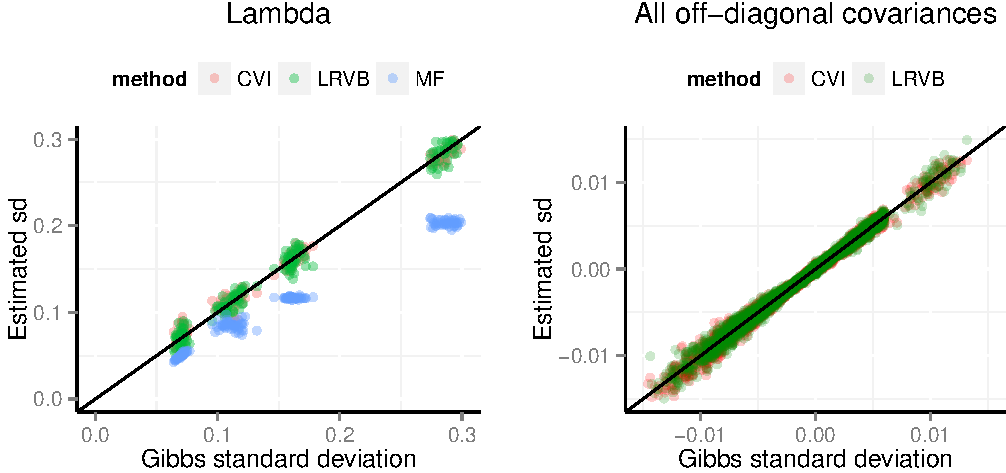
\includegraphics[width=0.7\textwidth]{img/mixture_gaussians.pdf}
  \caption{\label{fig:lrvb}Covariance estimates from
  copula variational inference (\gls{CVI}), mean-field (\gls{MF}), and
  linear response variational Bayes (\gls{LRVB}) to the ground truth
  (Gibbs samples). \gls{CVI} and \gls{LRVB} effectively capture dependence
  while \gls{MF} underestimates variance and forgets covariances.}
\end{figure}

We simulate $10,000$ samples with $K=2$ components and $P=2$
dimensional Gaussians. Figure \ref{fig:lrvb} displays estimates for
the standard deviations of $\mbLambda$ for 100 simulations, and plots
them against the ground truth using 500 effective Gibb samples. The
second plot displays all off-diagonal covariance estimates. Estimates
for $\mbmu$ and $\mbpi$ indicate the same pattern and are given in the
supplement.

When initializing at the true mean-field parameters, both \gls{CVI}
and \gls{LRVB} achieve consistent estimates of the posterior variance. \gls{MF} underestimates the variance, which is a well-known
limitation~\citep{wainwright2008graphical}. Note that
because the \gls{MF} estimates are initialized at the truth, \gls{CVI}
converges to the true posterior upon one step of fitting the copula. It does not require alternating more steps.

\Gls{CVI} is more robust than \gls{LRVB}. As a toy demonstration, we
analyze the MNIST data set of handwritten digits, using 12,665
training examples and 2,115 test examples of 0's and 1's. We perform
"unsupervised" classification, i.e., classify without using training
labels: we apply a mixture of Gaussians to cluster, and then classify
a digit based on its membership assignment. \gls{CVI} reports a test
set error rate of 0.06, whereas \gls{LRVB} ranges between 0.06 and
0.32 depending on the mean-field estimates. \gls{LRVB} and similar
higher order mean-field methods correct an existing \gls{MF}
solution---it is thus sensitive to local optima and the general
quality of that solution. On the other hand, \gls{CVI} re-adjusts both
the \gls{MF} and copula parameters as it fits, making it more robust
to initialization.

\subsection{Latent space model}
\label{subsec:latent}

We next study inference on the latent space
model~\citep{hoff2001latent}, a Bernoulli latent factor model for
network analysis. Each node in an $N$-node network is associated with
a $P$-dimensional latent variable $\mbz\sim N(\mbmu,\mbLambda^{-1})$.
Edges between pairs of nodes are observed with high probability if the
nodes are close to each other in the latent space. Formally, an edge
for each pair $(i,j)$ is observed with probability $\mathrm{logit}(p)=
\theta - |\mbz_i - \mbz_j|$, where $\theta$ is a model parameter.

We generate an $N=100,000$ node network with latent node attributes
from a $P=10$ dimensional Gaussian. We learn the posterior of the
latent attributes in order to predict the likelihood of held-out
edges. \gls{MF} applies independent factors on $\mbmu,
\mbLambda,\theta$ and $\mbz$, \gls{LRVB} applies a correction, and
\gls{CVI} uses the fully dependent variational distribution. Table
\ref{table:latent} displays the likelihood of held-out edges and runtime. We also attempted Hamiltonian Monte Carlo but it did not
converge after five hours.

\Gls{CVI} dominates other methods in accuracy upon convergence, and
the copula estimation without refitting (2 steps) already dominates
\gls{LRVB} in both runtime and accuracy. We note however that
\gls{LRVB} requires one to invert a
$\mathcal{O}(NK^3)\times\mathcal{O}(NK^3)$ matrix. We can better scale
the method and achieve faster estimates than \gls{CVI} if we applied
stochastic approximations for the inversion. However, \gls{CVI} always
outperforms \gls{LRVB} and is still fast on this 100,000 node network.

\begin{table}[t]
  \centering
  \begin{tabular}{lll}
  \toprule
  Variational inference methods & Predictive Likelihood & Runtime\\
  \midrule
  {Mean-field} & -383.2 & 15 min.\\
  \gls{LRVB} & -330.5 & 38 min.\\
  \gls{CVI} (2 steps) & -303.2 & 32 min.\\
  \gls{CVI} (5 steps) & -80.2 & 1 hr. 17 min.\\
  \gls{CVI} (converged) & -50.5 & 2 hr.\\
  \bottomrule
  \end{tabular}
  \captionof{table}{\label{table:latent}Predictive likelihood on the
  latent space model. Each \gls{CVI} step either refits the mean-field
  or the copula. \gls{CVI} converges in roughly 10 steps and already
  significantly outperforms both mean-field and \gls{LRVB} upon
  fitting the copula once (2 steps).}
\end{table}


%%% Local Variables:
%%% mode: latex
%%% TeX-master: "nips2015"
%%% End:


\section{Summary}
\label{sec:discussion}

We present operator variational objectives, a broad yet tractable
class of optimization problems for approximating posterior
distributions.  Operator objectives are built from an operator, a
family of test functions, and a distance function.  We outline the
connection between operator objectives and existing divergences such
as the KL divergence, and develop a new variational objective using
the Langevin-Stein operator.  In general, operator objectives produce
new ways of posing variational inference.

Given an operator objective, we develop a black box algorithm for
optimizing it and show which operators allow scalable optimization
through data subsampling.  Further, unlike the popular evidence lower
bound, not all operators explicitly depend on the approximating
density. This permits flexible approximating families, called
variational programs, where the distributional form is not
tractable. We demonstrate this approach on a mixture model and a
factor model of images.

There are several possible avenues for future directions such as
developing new variational objectives, adversarially learning~\citep{goodfellow2014generative} model parameters with operators, and
learning model parameters with operator variational objectives.


\parhead{Acknowledgments.}
This work is supported by NSF IIS-1247664,  ONR
N00014-11-1-0651, DARPA FA8750-14-2-0009, DARPA
N66001-15-C-4032, Adobe, NSERC PGS-D, Porter Ogden Jacobus Fellowship,
Seibel Foundation, and the Sloan Foundation. The authors would
like to thank Dawen Liang, Ben Poole, Stephan Mandt, Kevin Murphy, Christian
Naesseth,
and the anonymous reviews for their helpful feedback and comments.

\bibliographystyle{apalike}
{\small
\bibliography{bib}
}



\end{document}

